\section{SdLG Architecture and Controlled Modifications}
\label{sec:method}

SdLG-Exact is the reference recurrent-memory architecture. Sliding-window
attention (SWA) retains addressable recent features, and a normalized
full-matrix recurrence accumulates longer-range associations. Within every
reference block, SWA changes the representation before the associative stage
projects its queries, keys, and values. This differs from Griffin's
interleaving of recurrent and local-attention blocks across depth~\cite{de2024griffin};
SdLG has neither parallel local/global branches nor disjoint feature channels.

\begin{figure*}[t]
\centering
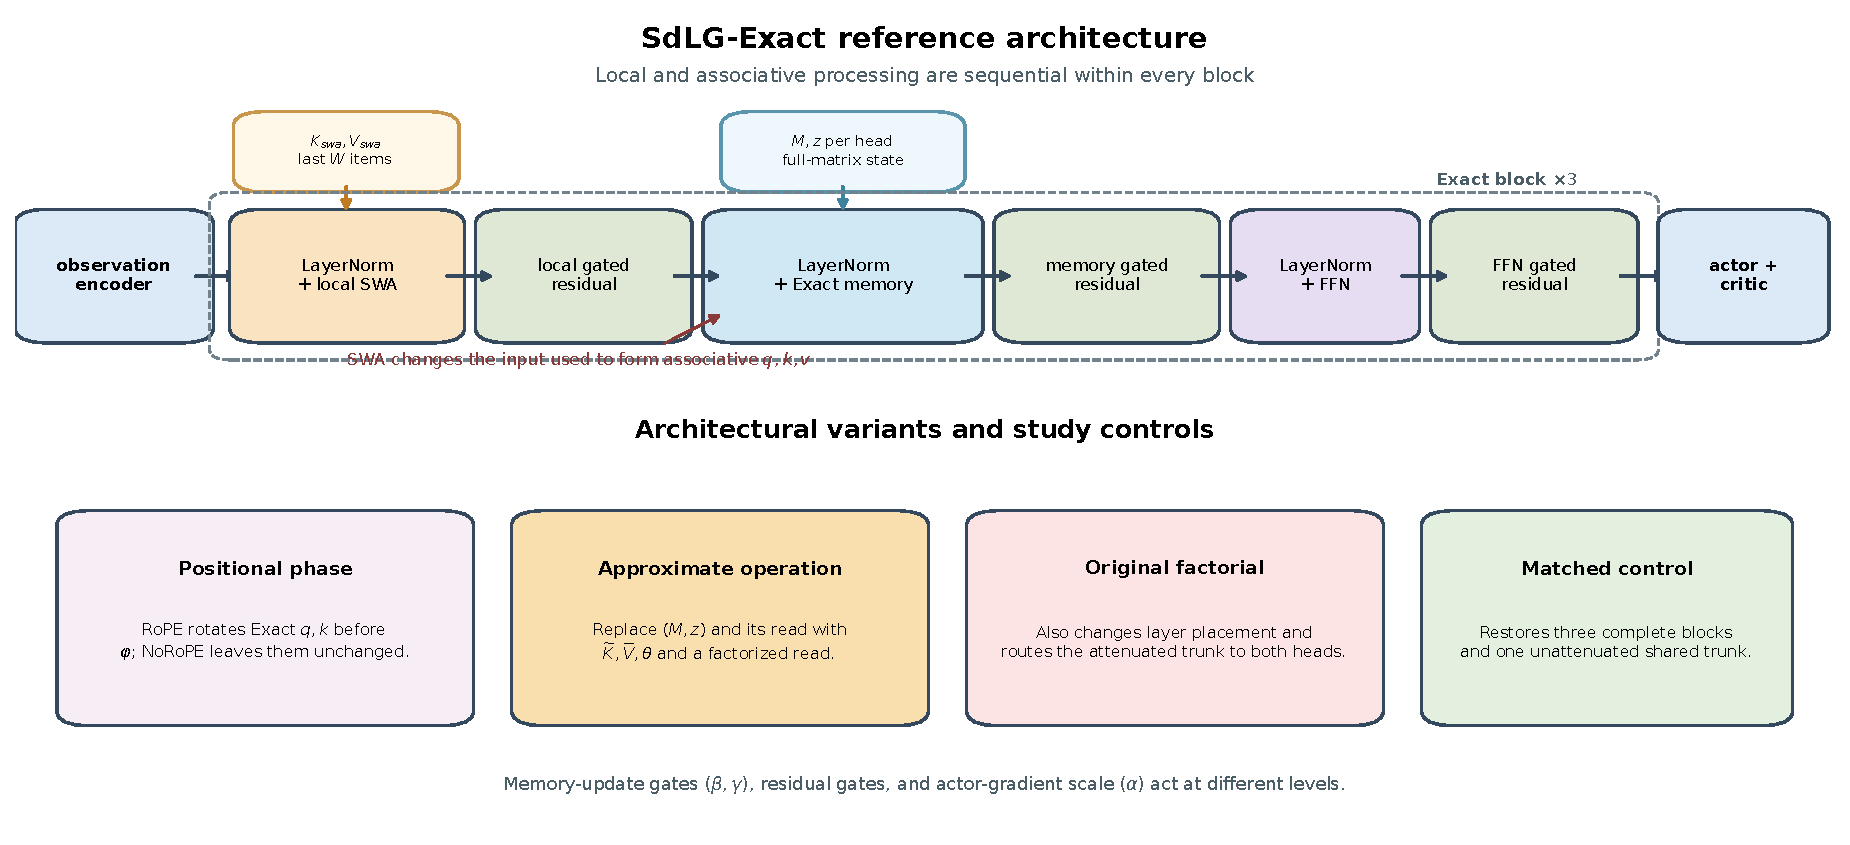
\includegraphics[width=0.92\textwidth]{plots/rebuilt/fig1_configuration_topologies}
\caption{\textbf{SdLG-Exact reference architecture and study-specific modifications.}
The large upper panel shows the implemented order within one Exact block:
pre-normalized SWA is fused by a gated residual, the full-matrix associative
stage reads and updates $(M,z)$ from the resulting representation and is fused
by a second gated residual, and an FFN is fused by a third. The tested T-Maze
reference repeats this complete block three times. The lower panel separates
modifications from the reference: positional phase changes query/key handling;
Approximate replaces the associative state, update, and read; the original
factorial also changes block placement and actor--critic routing; and the matched
comparison restores the reference block layout and common trunk.}
\label{fig:sdlg_flow}
\end{figure*}

\subsection{Reference Block and Processing Order}
Let $x_t^{(\ell)}$ denote the input to block $\ell$ at environment step $t$.
The block applies the following sequence:
\begin{align}
u_t^{(\ell)}
  &= \operatorname{SWA}\!\left(\operatorname{LN}(x_t^{(\ell)});
      K_{\mathrm{swa}},V_{\mathrm{swa}}\right),\\
x_{t,\mathrm{loc}}^{(\ell)}
  &= \mathcal{G}_{\mathrm{loc}}\!\left(x_t^{(\ell)},u_t^{(\ell)}\right),\\
(a_t^{(\ell)},M_t^{(\ell)},z_t^{(\ell)})
  &= \mathcal{A}_{\mathrm{Exact}}\!\left(\operatorname{LN}(x_{t,\mathrm{loc}}^{(\ell)});\right.\notag\\[-2pt]
  &\quad\left.M_{t-1}^{(\ell)},z_{t-1}^{(\ell)}\right),\\
x_{t,\mathrm{mem}}^{(\ell)}
  &= \mathcal{G}_{\mathrm{mem}}\!\left(x_{t,\mathrm{loc}}^{(\ell)},a_t^{(\ell)}\right),\\
f_t^{(\ell)}
  &= \operatorname{FFN}\!\left(\operatorname{LN}(x_{t,\mathrm{mem}}^{(\ell)})\right),\\
x_t^{(\ell+1)}
  &= \mathcal{G}_{\mathrm{ffn}}\!\left(x_{t,\mathrm{mem}}^{(\ell)},f_t^{(\ell)}\right).
\label{eq:exact_block_order}
\end{align}
Here $\mathcal{G}$ denotes a GTrXL-style GRU residual gate. The three gate
instances have separate parameters. The tested T-Maze Exact model applies three
of these complete blocks after a two-layer observation encoder, then sends the
final shared representation to the actor and critic heads.

This ordering resolves two different uses of the word \emph{parallel}. The
local and associative modules are sequential components of a block. Across the
time axis, however, the Exact affine recurrence is associative and can be
evaluated with a parallel prefix scan over a training chunk. Online execution
still updates it one environment step at a time.

\subsection{Local Sliding-Window Attention}
The local module stores $W$ projected key/value pairs and supplies a locally
processed residual stream to the associative recurrence. The execution used for the main results
uses circular buffer writes during one-step rollout and a chronological buffer
interpretation during sequence recomputation, without converting between the
two layouts. These paths therefore need not implement identical local windows.
Buffers carry across nonterminal rollout chunks and reset at episode boundaries;
the counter convention also distinguishes fresh initialization from an episode
reset. Appendix~\ref{app:original_local_execution} specifies these semantics.
The associative scan equivalence below concerns the associative recurrence for
given inputs, not equivalence of the entire policy across these execution paths.

\subsection{Gated Full-Matrix Associative Memory}
For each associative head, Exact maintains a matrix
$M_t\in\mathbb{R}^{d_k\times d_v}$ and a normalizer
$z_t\in\mathbb{R}^{d_k}$. From the locally processed representation it projects
$q_t,k_t\in\mathbb{R}^{d_k}$ and $v_t\in\mathbb{R}^{d_v}$, together with a scalar
write gate $\beta_t\in[0,1]$ and decay gate $\gamma_t\in(0,1]$. With the positive
feature map $\varphi(u)=1+\operatorname{ELU}(u)$, the state update is
\begin{align}
M_t &= \gamma_t M_{t-1}+\beta_t\varphi(k_t)v_t^\top,
\label{eq:matrix_recurrence}\\
z_t &= \gamma_t z_{t-1}+\beta_t\varphi(k_t),
\end{align}
and the query-dependent read is
\begin{equation}
y_t=\frac{\varphi(q_t)^\top M_t}
{\varphi(q_t)^\top z_t+\varepsilon},\qquad \varepsilon=10^{-6}.
\label{eq:query_retrieval}
\end{equation}
Exact therefore does not retain a list of all earlier keys and values or apply a
softmax over the full history. It retrieves from accumulated outer-product
associations, normalized by accumulated key features. Recall depends on the
learned representation, gate behavior, associative load, and interference. The
name \emph{Exact} identifies this full-matrix execution rather than promising
error-free recall or unlimited capacity. The implementation uses multiple
associative heads with separate matrix states and decay timescales.

At a new-episode observation, the continuation mask removes the preceding
episode's matrix and normalizer before the current write. Across a nonterminal
TBPTT boundary, $(M,z)$ and the SWA buffers are carried forward while their
computational graphs are detached. The associative composition proof, reset
semantics, and JAX implementation appear in Appendices~\ref{app:math_details}
and~\ref{app:implementation_details}.

\subsection{Three Distinct Control Mechanisms}
Three controls that act at different levels must not be conflated. First,
$\beta_t$ and $\gamma_t$ are \emph{memory-update gates}: they determine what is
written to the associative state and how much prior state is retained. Second,
$\mathcal{G}_{\mathrm{loc}}$, $\mathcal{G}_{\mathrm{mem}}$, and
$\mathcal{G}_{\mathrm{ffn}}$ are \emph{residual gates}: they determine how module
outputs alter the shared representation; they do not change Equations
\ref{eq:matrix_recurrence}--\ref{eq:query_retrieval}. Third, actor-gradient
routing is an \emph{optimization control} applied after the recurrent trunk. In
the dedicated Craftax Hybrid study it uses
\begin{equation}
x_{\mathrm{critic}}=x,\qquad
x_{\mathrm{actor}}=(1-\alpha)\operatorname{stopgrad}(x)+\alpha x,
\label{eq:ggs}
\end{equation}
so $\alpha$ scales the actor gradient entering the shared trunk without changing
the actor's forward input. It is not part of the Exact recurrence. SWA also
contains an internal output gate, but this belongs to the local module and is
separate from all three controls above.

\subsection{Controlled Modifications to the Reference}
The experiments change specific parts of the reference architecture:

\paragraph{Positional phase.}
When running-phase RoPE is enabled, the Exact branch rotates projected queries
and keys before applying $\varphi$; NoRoPE passes them through unchanged. This
changes positional handling, not the matrix state or the sequential block order.

\paragraph{Approximate associative execution.}
SdLG-Approximate replaces $(M,z)$ and Equations
\ref{eq:matrix_recurrence}--\ref{eq:query_retrieval} with factorized key and value
states $(\widetilde K,\widetilde V)$, phase state $\theta$, and a different
normalized read. It is therefore an alternative associative formulation, not
Exact with a smaller rank. Its equations and phase handling are given in
Appendix~\ref{app:approximate_execution}. Here $r$ is the total number of stored
factor rows per layer; Approximate has no Exact-style associative head axis and
shares its learned projections and update gates across rows. In the original T-Maze factorial,
Approximate additionally uses an alternating local--factorized--local stack and
routes an $\alpha=0.1$ attenuated representation to both PPO heads. That study
compares complete configurations rather than isolating associative rank. This
two-head attenuation differs from the actor-only gradient routing used in the
dedicated Craftax actor-gradient-scale study.

\paragraph{Matched execution control.}
The matched T-Maze comparison places Exact and Approximate associative operations
inside the same three complete local--associative--gated-FFN blocks and uses a
common unattenuated actor--critic trunk ($\alpha=1$). It removes block-placement
and routing differences while retaining the formulations' distinct state,
update, read, effective state size, and numerical path.

\paragraph{Component interventions.}
The MiniGrid intervention compares SWA enabled with SWA bypassed via
\texttt{local\_mode="none"}.
The Hybrid configuration is the factorized Approximate core with local
processing and a shared actor--critic trunk. The Craftax intervention changes
its actor-gradient scale. These are study-specific modifications, not defining
properties of Exact.
